% --- LeWorldModel (LeWM) ---
% % % --- Part F: LeWorldModel (Maes et al., arXiv:2603.19312) ---
\begin{frame}[t]{LeWorldModel (LeWM): Motivation}
  \centering
  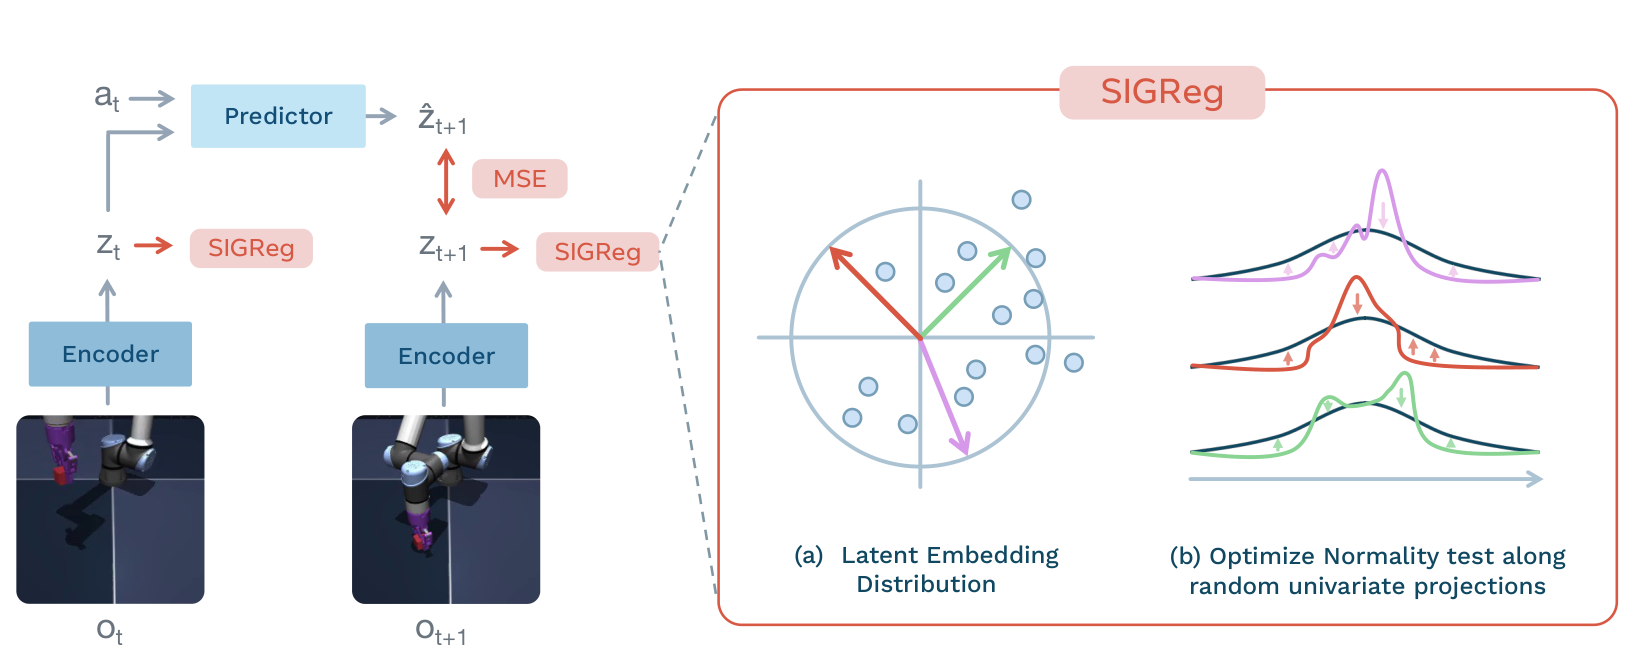
\includegraphics[width=0.82\linewidth,height=0.52\textheight,keepaspectratio]{images/world-models/leworldmodel_arxiv2603_fig1_training_pipeline_crop.png}\\[-0.08em]
  {\scriptsize Image credit: Maes et al., \href{https://arxiv.org/pdf/2603.19312v1.pdf}{LeWorldModel (arXiv:2603.19312)}.}
  \begin{itemize}\itemsep0.2em\footnotesize
    \item \textbf{LeWorldModel (LeWM):} a JEPA-style world model trained \textbf{end-to-end from raw pixels}, presented as the first to do so with only two loss terms.
    \item The two terms: a next-latent \textbf{prediction loss} and \textbf{SIGReg}, a regularizer that pushes latents toward a Gaussian distribution.
    \item This replaces the EMA / stop-gradient machinery of earlier JEPA recipes, with a stability and anti-collapse argument (as claimed in the paper).
  \end{itemize}
\end{frame}

\begin{frame}[t]{LeWorldModel (LeWM): Architecture}
  \centering
  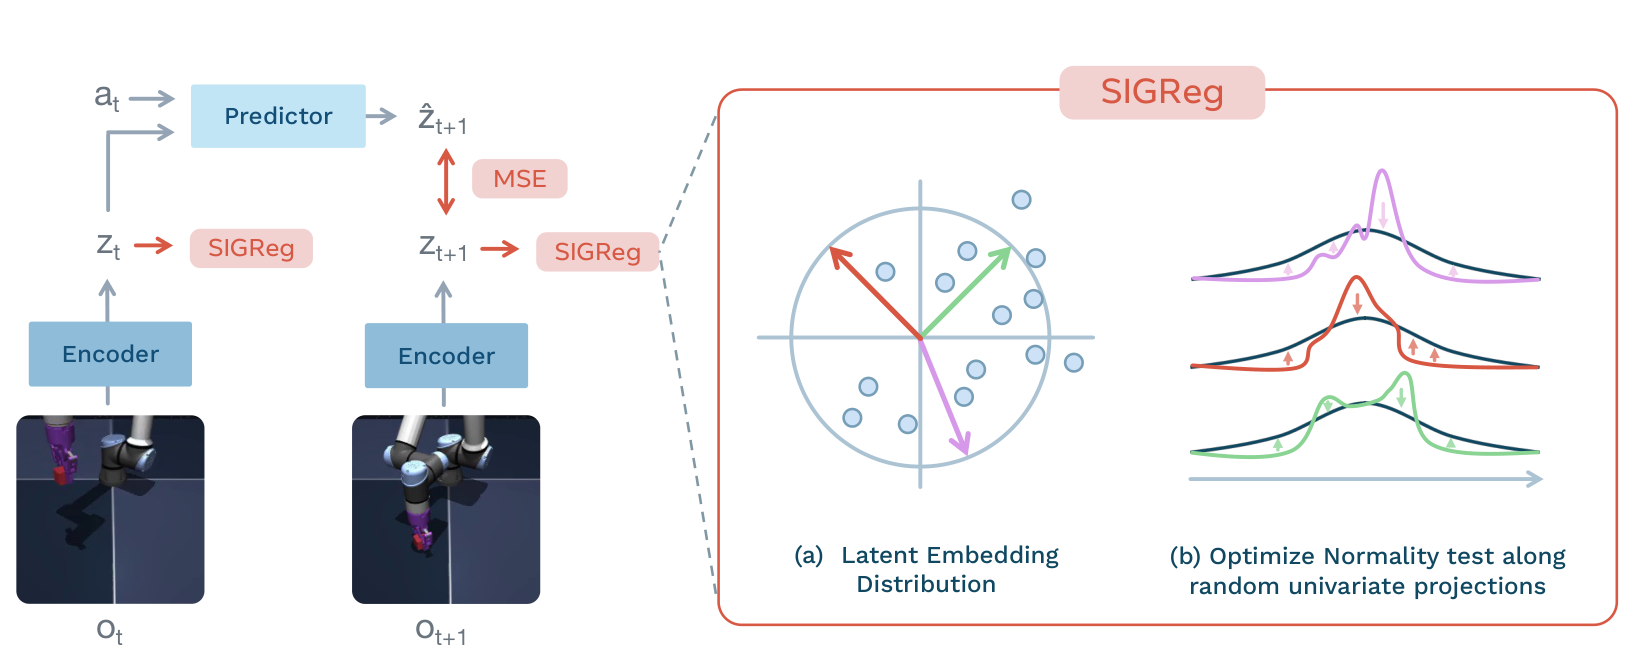
\includegraphics[width=0.82\linewidth,height=0.58\textheight,keepaspectratio]{images/world-models/leworldmodel_arxiv2603_fig1_training_pipeline_crop.png}\\[-0.08em]
  {\scriptsize Image credit: Maes et al., \href{https://arxiv.org/pdf/2603.19312v1.pdf}{LeWorldModel (arXiv:2603.19312)}.}
  \begin{itemize}\itemsep0.20em\footnotesize
    \item \textbf{Model Architecture.} LeWM consists of an encoder (mapping frames to latent codes) and a predictor (forecasting the next latent given the current latent and action).
    \item \textbf{Training Objective.} The model is trained end-to-end with a prediction loss plus a regularizer that encourages Gaussian-distributed latents:
    \[
        \mathcal{L} = \mathcal{L}_\text{pred} + \lambda\,\mathrm{SIGReg}(Z)
    \]
  \end{itemize}  
\end{frame}

\begin{frame}[t]{LeWorldModel (LeWM): Latent Planning}
  \begin{figure}[t]
    \centering
    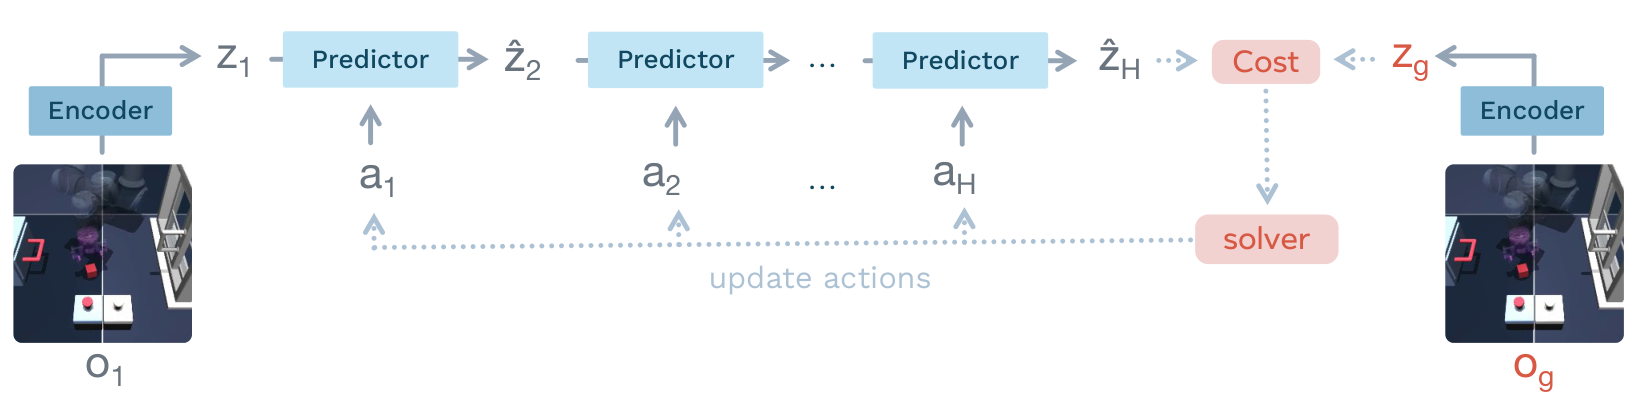
\includegraphics[width=0.98\linewidth,keepaspectratio]{images/world-models/leworldmodel_arxiv2603_fig4_latent_planning_p4.png}
    \caption*{\footnotesize
    \textbf{LeWorldModel Latent Planning.} Given an initial observation $o_1$ and a goal $o_g$, the world model learned performs planning in the LeWM latent space. The initial state embedding $z_1$ and the goal embedding $z_g$ are obtained from the encoder. The predictor then rolls out future latent states up to a horizon $H$. A latent cost between the final predicted state and the goal embedding guides a solver to optimize the action sequence. This prediction--optimization loop is repeated until convergence to a good plan candidate.
    }
  \end{figure}
\end{frame}

\begin{frame}[t]{LeWorldModel (LeWM): Results}
  \centering
  % Placeholder for bar chart image
  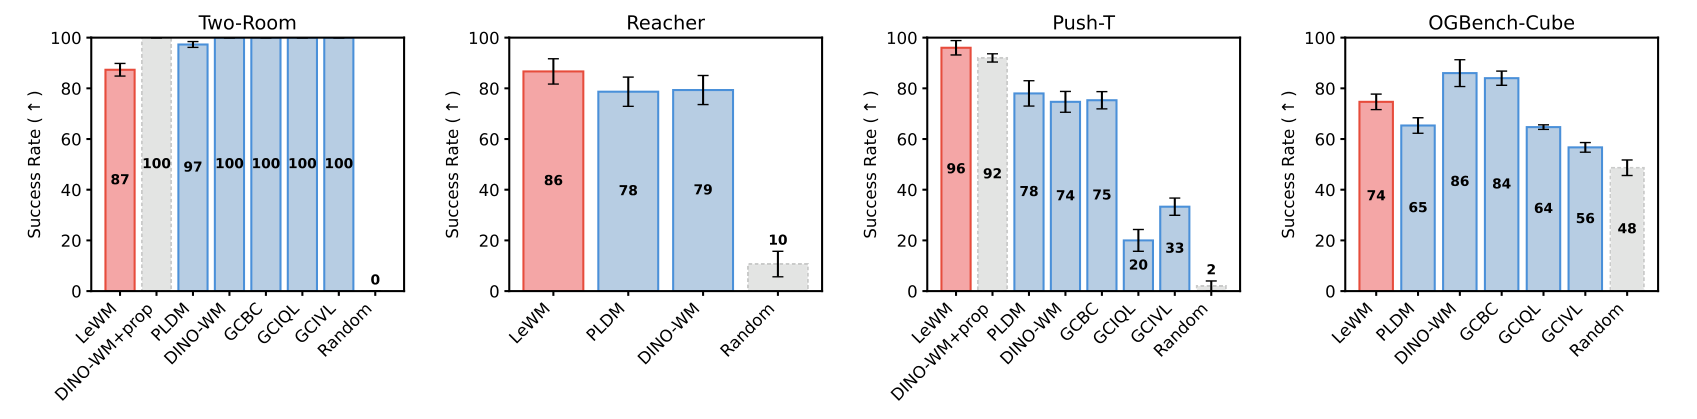
\includegraphics[width=0.97\linewidth]{images/world-models/leworldmodel_arxiv2603_fig6_planning_performance_p8.png}\\[0.4em]
  \footnotesize
  \textbf{Planning performance across environments} (Two-Room, Reacher, PushT, OGBench-Cube). LeWM outperforms PLDM and DINO-WM on PushT and Reacher. DINO-WM leads slightly on the visually complex 3D OGBench-Cube, and both baselines lead on the simple Two-Room task, where the paper suggests SIGReg's Gaussian pressure is a poor fit for a low-dimensional environment.
\end{frame}

% --- Synthesis across the lecture ---
\begin{frame}{Synthesis: Four Design Points}
  \begin{itemize}\itemsep0.26em
    \item \textbf{Ha \& Schmidhuber (V--M--C):} modular VAE + MDN-RNN + tiny controller; training inside the dream; a generative model with an evolution-trained policy.
    \item \textbf{PlaNet / Dreamer v1--v3:} ELBO-trained RSSM latents; CEM planning (PlaNet), then actor-critic learned in imagination (Dreamer); categorical latents and normalization for stability at scale.
    \item \textbf{V-JEPA 2 (+AC):} non-generative video SSL at scale; an action-conditioned head plus CEM planning brings it to robotics (JEPA lecture).
    \item \textbf{LeWM:} JEPA from pixels for control, with SIGReg replacing EMA recipes; a small model with fast latent planning, and a good code-first reference for course projects.
  \end{itemize}
\end{frame}

% --- Synthesis ---
% \begin{frame}{Cheat Sheet}
%   \begin{itemize}\itemsep0.26em
%     \item \textbf{Ha 2018 (V--M--C):} modular VAE+MDN-RNN+controller; train-in-the-dream; exposes \textbf{generative} world-model design patterns and RPG issues.
%     \item \textbf{RSSM / DreamerV3:} \textbf{ELBO-trained} latent dynamics + actor--critic on imagined rollouts; categorical latents, symlog, and strong scaling curves.
%     \item \textbf{V-JEPA / V-JEPA\,2 / 2.1:} \textbf{non-generative} video SSL at scale; add \textbf{AC} heads or LLM alignment for robotics / VQA; different training stack than Dreamer.
%     \item \textbf{LeWM:} \textbf{JEPA-from-pixels control} with \textbf{SIGReg} instead of EMA/stop-grad recipes---good code-first reference for MSc projects.
%   \end{itemize}
% \end{frame}
